\documentclass[margin=5mm]{standalone}
\usepackage[utf8]{inputenc}
\usepackage{amsmath}
\usepackage{amsfonts}
\usepackage{amssymb}
\usepackage{graphicx}
\usepackage{tikz}
% \usepackage{mathpazo}
\usepackage[scaled=0.92]{helvet}

\usetikzlibrary{positioning, calc}
\usetikzlibrary{shadows.blur}
\usetikzlibrary{shapes, positioning, calc, decorations.markings, arrows.meta}

\tikzstyle{arrow}=[line width=1mm,draw=black, -{Triangle[length=3mm]}, postaction={draw, line width=2mm, shorten >=1mm, -}]
\tikzstyle{line}=[line width=2mm,draw=black]
\tikzstyle{component}=[rectangle, draw, fill=white, ultra thick, minimum height=1.5cm, minimum width = 2cm, align=center]
% \tikzstyle{component}=[rectangle, draw, fill=white, thick, minimum height=1.5cm, minimum width = 2cm, blur shadow={shadow blur steps=5}, align=center]

\begin{document}
    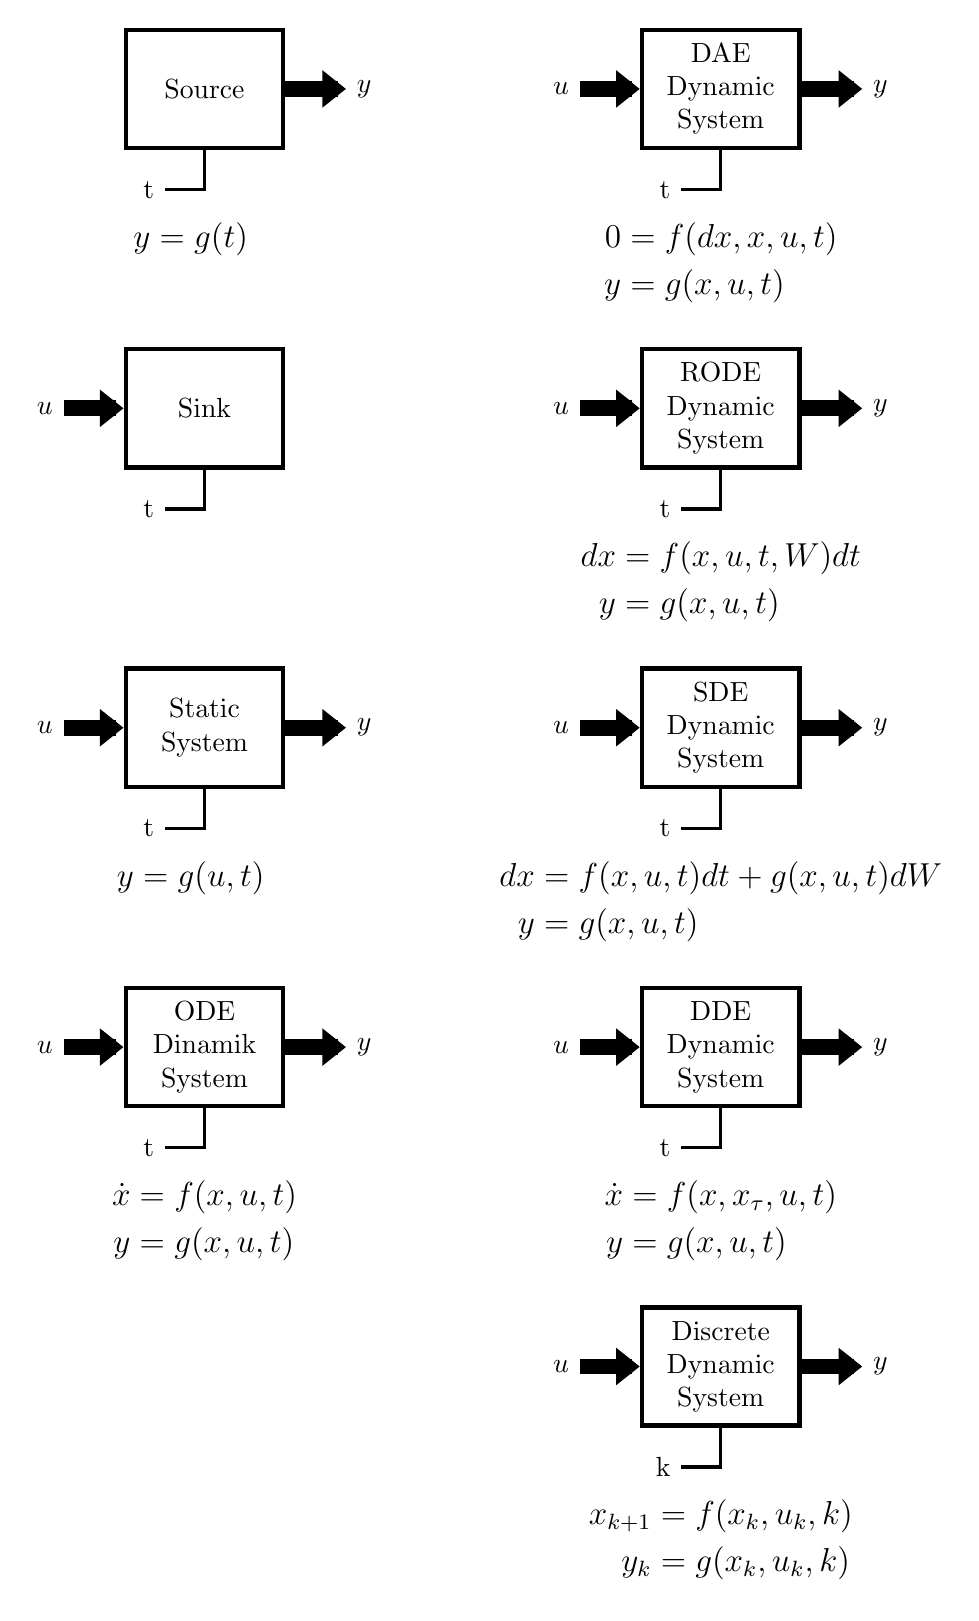
\begin{tikzpicture}[node distance = 2.5cm, very thick]
        % Draw the blocks
        \node[component](source){Source};
        % \node[xshift=-1cm] (in source) at (source.west) {$u$};
        \node[xshift=1cm] (out source) at (source.east) {$y$};
        % \draw[arrow] (in source) -- (source.west);
        \draw[arrow] (source.east) -- (out source);
        \node[below = 0.75cm of source]{\large
            $\begin{aligned}
                y &= g(t)
             \end{aligned}$
        };
        
        \node[component, below = of source](sink){Sink};
        \node[xshift=-1cm] (in sink) at (sink.west) {$u$};
        % \node[xshift=1cm] (out sink) at (sink.east) {$y$};
        \draw[arrow] (in sink) -- (sink.west);
        % \draw[arrow] (sink.east) -- (out sink);
        % \node[below = 0.1cm of sink]{
        %     $\begin{aligned}
        %         y &= g(t) \\
        %         y &= g(t)
        %      \end{aligned}$
        % };

        \node[component, below = of sink](static system){Static \\ System};
        \node[xshift=-1cm] (in static system) at (static system.west) {$u$};
        \node[xshift=1cm] (out static system) at (static system.east) {$y$};
        \draw[arrow] (in static system) -- (static system.west);
        \draw[arrow] (static system.east) -- (out static system);
        \node[below = 0.75cm of static system]{\large
            $\begin{aligned}
                y &= g(u, t)
             \end{aligned}$
        };


        \node[component, below = of static system](ode system){ODE \\ Dinamik \\ System};
        \node[xshift=-1cm] (in ode system) at (ode system.west) {$u$};
        \node[xshift=1cm] (out ode system) at (ode system.east) {$y$};
        \draw[arrow] (in ode system) -- (ode system.west);
        \draw[arrow] (ode system.east) -- (out ode system);
        \node[below = 0.75cm of ode system]{ \large
            $\begin{aligned}
                \dot{x} &= f(x, u, t) \\
                y &= g(x, u, t)
             \end{aligned}$
        };

        \node[component, right = of source, xshift=2cm](dae system){DAE \\ Dynamic \\ System};
        \node[xshift=-1cm] (in dae system) at (dae system.west) {$u$};
        \node[xshift=1cm] (out dae system) at (dae system.east) {$y$};
        \draw[arrow] (in dae system) -- (dae system.west);
        \draw[arrow] (dae system.east) -- (out dae system);
        \node[below = 0.75cm of dae system]{\large
            $\begin{aligned}
                0 &= f(dx, x, u, t) \\
                y &= g(x, u, t)
             \end{aligned}$
        };

        \node[component, below = of dae system](rode system){RODE \\ Dynamic \\ System};
        \node[xshift=-1cm] (in rode system) at (rode system.west) {$u$};
        \node[xshift=1cm] (out rode system) at (rode system.east) {$y$};
        \draw[arrow] (in rode system) -- (rode system.west);
        \draw[arrow] (rode system.east) -- (out rode system);
        \node[below = 0.75cm of rode system]{ \large
            $\begin{aligned}
                dx &= f(x, u, t, W)dt \\
                y &= g(x, u, t)
             \end{aligned}$
        };

        \node[component, below = of rode system](sde system){SDE \\ Dynamic \\ System};
        \node[xshift=-1cm] (in sde system) at (sde system.west) {$u$};
        \node[xshift=1cm] (out sde system) at (sde system.east) {$y$};
        \draw[arrow] (in sde system) -- (sde system.west);
        \draw[arrow] (sde system.east) -- (out sde system);
        \node[below = 0.75cm of sde system]{\large
            $\begin{aligned}
                dx &= f(x, u, t)dt + g(x, u, t)dW \\
                y &= g(x, u, t)
             \end{aligned}$
        };

        \node[component, below = of sde system](dde system){DDE \\ Dynamic \\ System};
        \node[xshift=-1cm] (in dde system) at (dde system.west) {$u$};
        \node[xshift=1cm] (out dde system) at (dde system.east) {$y$};
        \draw[arrow] (in dde system) -- (dde system.west);
        \draw[arrow] (dde system.east) -- (out dde system);
        \node[below = 0.75cm of dde system]{\large
            $\begin{aligned}
                \dot{x} &= f(x, x_\tau, u, t)\\
                y &= g(x, u, t)
             \end{aligned}$
        };

        \node[component, below = of dde system](discrete system){Discrete \\ Dynamic \\ System};
        \node[xshift=-1cm] (in discrete system) at (discrete system.west) {$u$};
        \node[xshift=1cm] (out discrete system) at (discrete system.east) {$y$};
        \draw[arrow] (in discrete system) -- (discrete system.west);
        \draw[arrow] (discrete system.east) -- (out discrete system);
        \node[below = 0.75cm of discrete system]{\large
            $\begin{aligned}
                x_{k + 1} &= f(x_k, u_k, k)\\
                y_k &= g(x_k, u_k, k)
             \end{aligned}$
        };

        \def\points{source, sink, static system, ode system, dae system, rode system, sde system, dde system}
        \foreach \p in \points {
            \draw (\p.south) |- ++(-0.5, -0.5) node[anchor=east]{t};
        }
        \draw (discrete system.south) |- ++(-0.5, -0.5) node[anchor=east]{k};

    \end{tikzpicture}
\end{document}